\chapter{The Eye and Its Photoreceptors}\label{ch:g11:the-eye}

On a moonless night, away from any lamp, you can see the path but not
its colours; a friend's red jacket is a grey shape. Look straight at a
faint star and it vanishes; look slightly to one side and it
reappears. Both oddities come from the retina, the thin sheet at the
back of the \omterm{def:g11:the-eye:parts}{eye} where light becomes a nerve signal: two kinds of
receptor \omterm{def:g10:cells-common-unit:cell}{cell}, unequally distributed, one of them blind to colour and
the other blind in the dark. This chapter takes the \omterm{def:g11:the-eye:parts}{eye} apart from the
cornea to the optic nerve, and reads, in the \omterm{def:g10:universal-dna:gene}{genes} of the retina's
pigments, a piece of our evolutionary history.

\section{The eye as an optical instrument}

\begin{definition}[The parts of the eye]\label{def:g11:the-eye:parts}
The \emph{eye}\index{eye} is a globe about \qty{24}{mm} across. Light
enters through the transparent \emph{cornea}, passes the \emph{pupil}
--- the opening in the coloured \emph{iris}, which widens in the dark
and narrows in bright light --- and the \emph{lens}, crosses the clear
jelly of the \emph{vitreous body}, and reaches the \emph{retina}, the
light-sensitive layer lining the back of the globe. Cornea and lens
together form, on the retina, a small inverted image of the scene; the
lens, whose curvature muscles can change, adjusts the focus from
distant to near objects (\emph{accommodation}). The
\emph{optic nerve} leaves the back of the eye carrying the retina's
signals to the brain.
\end{definition}

\begin{omfigure}
\begin{tikzpicture}
  \node[anchor=south west, inner sep=0] (img) at (0,0)
    {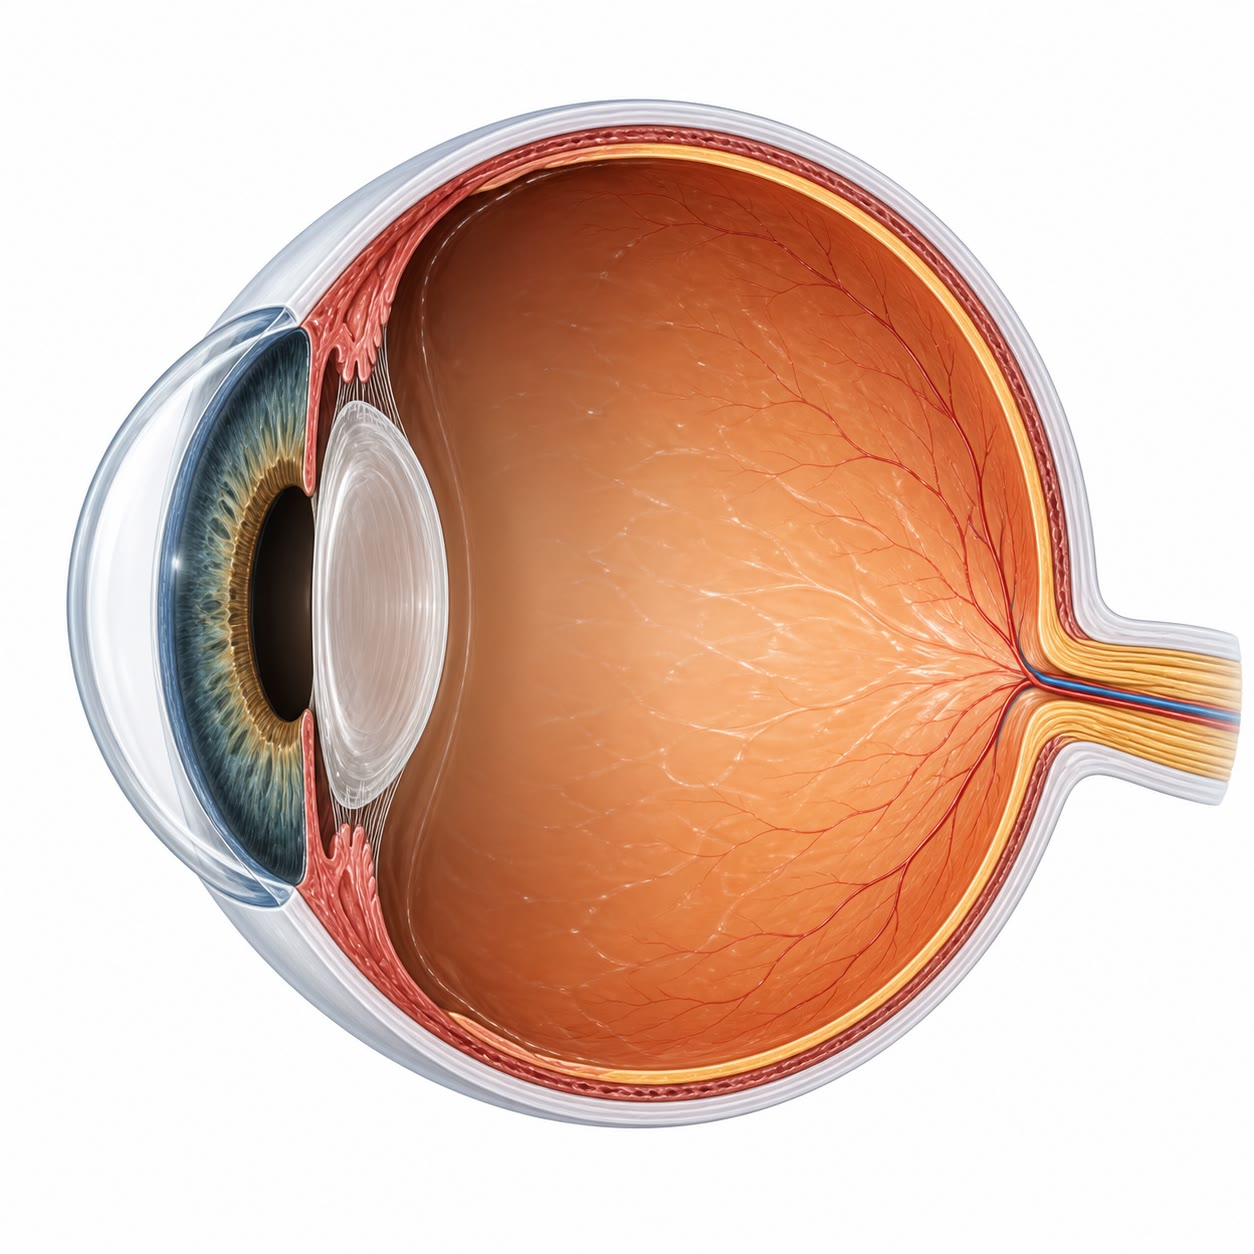
\includegraphics[width=0.46\linewidth]{images/book2/ai/fig-eye-cutaway.jpg}};
  \begin{scope}[x={(img.south east)}, y={(img.north west)},
      every node/.style={font=\small}]
    \draw[omDef, thick] (0.10,0.55) -- (-0.05,0.80) node[left] {cornea};
    \draw[omDef, thick] (0.18,0.36) -- (-0.05,0.20) node[left] {iris and pupil};
    \draw[omDef, thick] (0.26,0.50) -- (-0.05,0.50) node[left] {lens};
    \draw[omDef, thick] (0.55,0.50) -- (0.55,-0.06) node[below] {vitreous body};
    \draw[omDef, thick] (0.83,0.76) -- (1.05,0.88) node[right] {retina};
    \draw[omDef, thick] (0.95,0.40) -- (1.05,0.20) node[right] {optic nerve};
  \end{scope}
\end{tikzpicture}

{\small The \omterm{def:g11:the-eye:parts}{eye} in horizontal section. The cornea and the lens focus
the light; the retina, at the back, converts it into signals that
leave through the optic nerve.}
\end{omfigure}

\begin{example}[Focus, and its faults]\label{ex:g11:the-eye:focus}
A relaxed \omterm{def:g11:the-eye:parts}{eye} focuses distant objects on the retina; to read at
\qty{25}{cm} the lens must bulge. An \omterm{def:g11:the-eye:parts}{eye} slightly too long focuses
distant objects in front of the retina --- short sight, corrected by a
diverging spectacle lens; an \omterm{def:g11:the-eye:parts}{eye} too short, or a lens that has
stiffened with age, cannot bring near objects to focus --- long sight,
corrected by a converging lens. In each case the retina is intact:
the fault is optical, and glasses put the image back where the
receptors are.
\end{example}

\section{The retina}

\begin{definition}[Photoreceptors]\label{def:g11:the-eye:photoreceptors}
The retina contains two kinds of \emph{photoreceptor}\index{photoreceptor}
\omterm{def:g10:cells-common-unit:cell}{cells}, named for their shape. The \emph{rods}\index{rod (retina)},
about 120 million, respond to very dim light but all with the same
pigment: they give vision in shades of grey at night. The
\emph{cones}\index{cone (retina)}, about 6 million, need brighter
light and come in three types, each with a pigment most sensitive to
a different part of the spectrum: they give daylight vision and
colour. Each photoreceptor contains a \emph{photopigment} --- a
\omterm{def:g11:gene-expression:protein}{protein}, an \emph{opsin}\index{opsin}, holding a small
light-absorbing molecule derived from vitamin A --- whose change of
shape on absorbing a photon starts the \omterm{def:g10:cells-common-unit:cell}{cell}'s electrical response.
\end{definition}

\begin{omfigure}
\begin{tikzpicture}[font=\small, >=Stealth, line cap=round]
  % layers from front (left) to back (right); light comes from the left
  \draw[->, very thick, omProp] (-1.6,1.2) -- (-0.3,1.2) node[pos=0, above, omProp] {light};
  % ganglion cells
  \foreach \y in {2.4,1.2,0.0} { \draw[thick, fill=omDef!25] (0.4,\y) circle (0.28); \draw[thick, omDef] (0.12,\y) -- (-0.6,\y) -- (-0.6,-1.4); }
  \node[anchor=north, align=center] at (0.4,-0.5) {ganglion\\ cells};
  \draw[->, thick, omDef] (-0.6,-1.4) -- (-0.6,-2.0) node[below, align=center] {to the\\ optic nerve};
  % bipolar cells
  \foreach \y in {2.4,1.2,0.0} { \draw[thick, fill=omMeth!25] (2.2,\y) ellipse (0.22 and 0.36); \draw[thick] (0.68,\y) -- (1.98,\y); \draw[thick] (2.42,\y) -- (3.1,\y); }
  \node[anchor=north, align=center] at (2.2,-0.5) {bipolar\\ cells};
  % photoreceptors: rods (tall rectangles) and cones (triangles)
  \foreach \y in {2.4,0.0} { \draw[thick, fill=gray!30] (3.1,\y-0.18) rectangle (5.0,\y+0.18); \node[font=\scriptsize] at (4.05,\y) {rod}; }
  \draw[thick, fill=omThm!25] (3.1,1.2-0.22) -- (5.0,1.2-0.08) -- (5.0,1.2+0.08) -- (3.1,1.2+0.22) -- cycle;
  \node[font=\scriptsize] at (4.05,1.2) {cone};
  \node[anchor=north, align=center] at (4.5,-0.5) {photoreceptors\\ (pigment at tip)};
  % pigment epithelium
  \fill[gray!60] (5.2,-0.2) rectangle (5.6,2.8);
  \node[anchor=west, align=left] at (5.7,1.2) {dark layer\\ absorbing\\ stray light};
  \node[anchor=south, align=center, font=\scriptsize] at (2.6,3.0) {the signal travels from right to left, against the light};
\end{tikzpicture}

{\small The retina, in section. Light crosses the transparent layers
of nerve \omterm{def:g10:cells-common-unit:cell}{cells} and reaches the \omterm{def:g11:the-eye:photoreceptors}{photoreceptors} at the back, whose
light-absorbing tips face away from it; the signal then travels
forward, from receptor to bipolar \omterm{def:g10:cells-common-unit:cell}{cell} to ganglion \omterm{def:g10:cells-common-unit:cell}{cell}, whose fibres
form the optic nerve.}
\end{omfigure}

\begin{proposition}[Organisation of the retina]\label{prop:g11:the-eye:organisation}
The \omterm{def:g11:the-eye:photoreceptors}{photoreceptors} lie at the back of the retina, against a dark
layer; the light must cross the other layers to reach them. Their
signals pass to \emph{bipolar \omterm{def:g10:cells-common-unit:cell}{cells}}, then to \emph{ganglion \omterm{def:g10:cells-common-unit:cell}{cells}},
whose long fibres --- about a million --- gather into the optic nerve.
The distribution is uneven: at the \emph{fovea}, the small central
pit the \omterm{def:g11:the-eye:parts}{eye} points at, there are only \omterm{def:g11:the-eye:photoreceptors}{cones}, packed tightly and each
connected to its own ganglion \omterm{def:g10:cells-common-unit:cell}{cell}, giving the sharpest vision; away
from the centre, \omterm{def:g11:the-eye:photoreceptors}{rods} dominate and many of them share one ganglion
\omterm{def:g10:cells-common-unit:cell}{cell}, giving sensitivity at the price of detail. Where the optic
nerve leaves, there are no receptors at all: the \emph{blind spot}.
\end{proposition}
\admitted

\begin{omfigure}
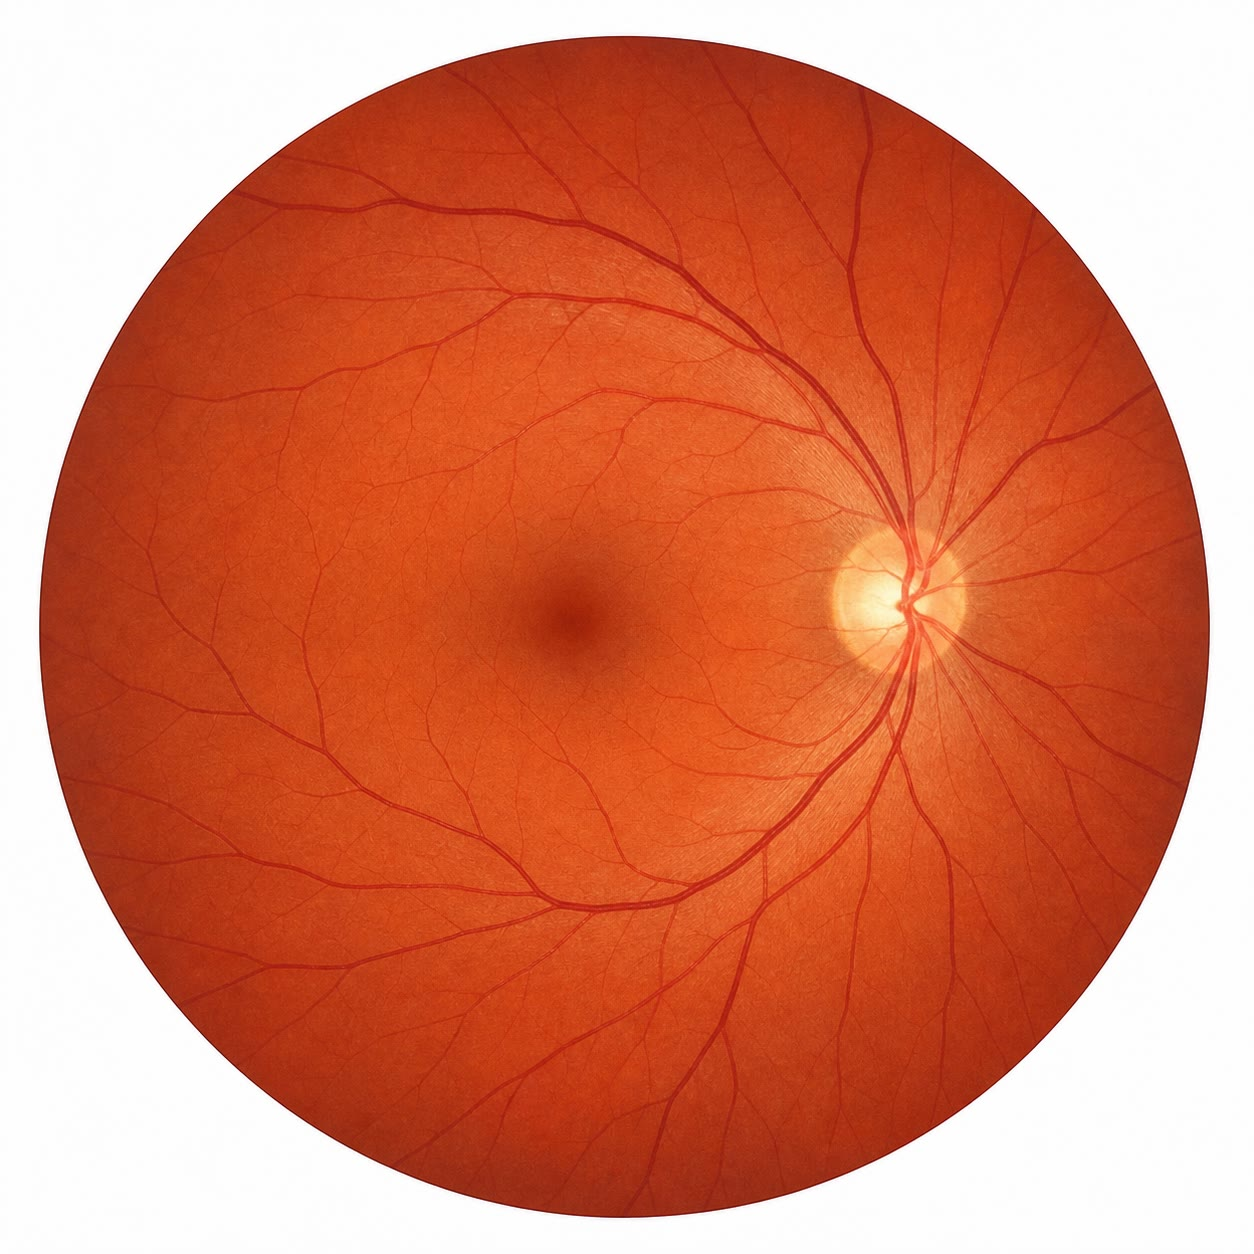
\includegraphics[width=0.42\linewidth]{images/book2/ai/g11-retina-fundus.jpg}

{\small The retina seen through the pupil with an ophthalmoscope: the
pale disc where the optic nerve leaves and the vessels enter (the blind
spot), and, darker and to one side, the fovea where \omterm{def:g11:the-eye:photoreceptors}{cones} are densest.}
\end{omfigure}

\begin{example}[The two oddities explained]\label{ex:g11:the-eye:oddities}
The faint star vanishes when looked at directly because the fovea has
only \omterm{def:g11:the-eye:photoreceptors}{cones}, which need more light than the star provides; looked at
sideways, its light falls on \omterm{def:g11:the-eye:photoreceptors}{rods}, which detect it. The jacket is grey
at night because the \omterm{def:g11:the-eye:photoreceptors}{rods} that see it have a single pigment: they can
report how much light, not which wavelength. Colour is a comparison
between the three cone types, and the \omterm{def:g11:the-eye:photoreceptors}{cones} are silent in the dark.
\end{example}

\section{Colour: three pigments}

\begin{proposition}[Colour vision]\label{prop:g11:the-eye:colour}
Each cone type contains one of three \omterm{def:g11:the-eye:photoreceptors}{opsins}, whose absorption peaks
near \qty{420}{nm} (S \omterm{def:g11:the-eye:photoreceptors}{cones}, blue), \qty{530}{nm} (M \omterm{def:g11:the-eye:photoreceptors}{cones}, green) and
\qty{560}{nm} (L \omterm{def:g11:the-eye:photoreceptors}{cones}, red). A given light excites the three types in
proportions that depend on its wavelength; the brain reads the colour
from those proportions. A person lacking one cone type confuses the
colours that type distinguished: without working L or M \omterm{def:g11:the-eye:photoreceptors}{cones}, red
and green are hard to tell apart --- \emph{red--green colour
blindness}, which affects about 8\% of men and 0.5\% of women.
\end{proposition}
\admitted

\begin{omfigure}
\begin{tikzpicture}
\begin{axis}[
  width=0.9\linewidth, height=5.8cm,
  axis x line=bottom, axis y line=left,
  xmin=380, xmax=700, ymin=0, ymax=110,
  xlabel={wavelength (nm)}, ylabel={absorption (\% of peak)},
  xlabel style={font=\small, at={(axis description cs:0.5,-0.12)}, anchor=north},
  ylabel style={font=\small},
  tick label style={font=\small}, xtick={400,450,500,550,600,650,700}, ytick={0,50,100},
  legend style={at={(0.5,-0.3)}, anchor=north, legend columns=4, font=\small, draw=none},
]
\addplot[thick, omDef, smooth] coordinates {(380,40) (400,75) (420,100) (440,88) (460,55) (480,25) (500,8) (520,2) (540,0)};
\addplot[thick, gray, dashed, smooth] coordinates {(400,10) (430,35) (460,70) (480,90) (500,100) (520,90) (540,65) (560,38) (580,18) (600,7) (620,2) (640,0)};
\addplot[thick, omMeth, smooth] coordinates {(420,5) (450,20) (480,50) (510,85) (530,100) (550,90) (570,65) (590,38) (610,18) (630,7) (650,2) (670,0)};
\addplot[thick, omThm, smooth] coordinates {(440,5) (470,18) (500,40) (530,80) (560,100) (580,92) (600,70) (620,42) (640,20) (660,8) (680,3) (700,1)};
\legend{S cones (blue), rods, M cones (green), L cones (red)}
\end{axis}
\end{tikzpicture}

{\small Absorption of the four photopigments against wavelength.
Each is broad and they overlap; a yellow light of \qty{580}{nm}
excites the L \omterm{def:g11:the-eye:photoreceptors}{cones} strongly, the M \omterm{def:g11:the-eye:photoreceptors}{cones} moderately and the S \omterm{def:g11:the-eye:photoreceptors}{cones}
not at all --- that ratio is what "yellow" means to the brain.}
\end{omfigure}

\begin{example}[Reading the curves]\label{ex:g11:the-eye:curves}
Light of \qty{500}{nm}: S \omterm{def:g11:the-eye:photoreceptors}{cones} at 8\%, M at 75\%, L at 40\% ---
seen as blue-green. Light of \qty{620}{nm}: S at 0, M at 10\%, L at
42\% --- red. A person without L \omterm{def:g11:the-eye:photoreceptors}{cones} receives, for both, only an S
and an M value, and the second light gives S~0, M~10: barely
distinguishable from a dim green. The colours that the missing type
would have told apart collapse into one.
\end{example}

\section{The opsin genes: a family with a history}

\begin{proposition}[Genes of the opsins]\label{prop:g11:the-eye:genes}
Each \omterm{def:g11:the-eye:photoreceptors}{opsin} is encoded by its own \omterm{def:g10:universal-dna:gene}{gene}. The \omterm{def:g11:the-eye:photoreceptors}{S-opsin} \omterm{def:g10:universal-dna:gene}{gene} lies on an
ordinary \omterm{def:g11:cell-cycle-mitosis:chromosome}{chromosome}; the M- and \omterm{def:g11:the-eye:photoreceptors}{L-opsin} \omterm{def:g10:universal-dna:gene}{genes} lie side by side on the
X \omterm{def:g11:cell-cycle-mitosis:chromosome}{chromosome}. The L and M \omterm{def:g11:gene-expression:protein}{proteins} differ at only 15 of their 364
\omterm{def:g10:chemistry-of-life:families}{amino acids} (96\% identical), the S \omterm{def:g11:gene-expression:protein}{protein} at more than half of its
positions from either. Being on the X, a non-working M or L \omterm{def:g10:universal-dna:gene}{allele} is
expressed in every male who carries it and only in females carrying
two --- the pattern of \cref{ch:g11:genes-and-disease}, and the reason
red--green colour blindness is sixteen times commoner in men.
\end{proposition}
\admitted

\begin{proposition}[A family of genes from duplications]\label{prop:g11:the-eye:family}
The three \omterm{def:g11:the-eye:photoreceptors}{opsin} \omterm{def:g10:universal-dna:gene}{genes}, and the rod pigment's, are versions of one
ancestral \omterm{def:g10:universal-dna:gene}{gene} copied by \emph{duplication} and then diverged by
\omterm{def:g11:mutations:mutation}{mutation}. Their degrees of similarity date the copies: the S and
L/M lines separated very early in \omterm{def:g10:common-ancestry:bodyplan}{vertebrate} history, some 500 million
years ago; the L and M \omterm{def:g10:universal-dna:gene}{genes} arose from one duplication about 30 to
40 million years ago in the ancestor of the Old World primates, whose
descendants --- monkeys, apes, humans --- have three cone types while
most other mammals have two.
\end{proposition}
\begin{proof}[Evidence]
Sequence comparison: the L and M \omterm{def:g10:universal-dna:gene}{genes} are 96\% identical and adjacent
on the X --- the signature of a recent tandem duplication; each is
about 43\% identical to the S \omterm{def:g10:universal-dna:gene}{gene}, and all three about 40\%
identical to the rod \omterm{def:g11:the-eye:photoreceptors}{opsin} \omterm{def:g10:universal-dna:gene}{gene}, the more distant copies. Dogs, cattle
and most mammals have only one X-linked \omterm{def:g11:the-eye:photoreceptors}{opsin} \omterm{def:g10:universal-dna:gene}{gene}, in the position
where primates have two; New World monkeys have one, with several
\omterm{def:g10:universal-dna:gene}{alleles}, and only females carrying two different \omterm{def:g10:universal-dna:gene}{alleles} see three
colours. The \omterm{def:g10:universal-dna:gene}{gene} count matches the cone count in each lineage, and
the tree of the \omterm{def:g10:universal-dna:gene}{genes} matches the tree of the \omterm{def:g10:biodiversity-scales:species}{species}.
\end{proof}

\begin{omfigure}
\begin{tikzpicture}[font=\small, line cap=round]
  % gene tree: root -> (rod opsin) ; (S) ; (L/M split)
  \draw[thick] (0,2) -- (1.5,2);
  \draw[thick] (1.5,2) -- (1.5,3.4) -- (9,3.4);
  \draw[thick] (1.5,2) -- (1.5,0.6) -- (3.2,0.6);
  \draw[thick] (3.2,0.6) -- (3.2,1.8) -- (9,1.8);
  \draw[thick] (3.2,0.6) -- (3.2,-0.6) -- (7.6,-0.6);
  \draw[thick] (7.6,-0.6) -- (7.6,0.2) -- (9,0.2);
  \draw[thick] (7.6,-0.6) -- (7.6,-1.4) -- (9,-1.4);
  \fill[omThm] (1.5,2) circle (2.5pt); \fill[omThm] (3.2,0.6) circle (2.5pt); \fill[omThm] (7.6,-0.6) circle (2.5pt);
  \node[anchor=west] at (9.1,3.4) {rod opsin (rhodopsin)};
  \node[anchor=west] at (9.1,1.8) {S opsin (blue cones)};
  \node[anchor=west] at (9.1,0.2) {M opsin (green cones)};
  \node[anchor=west] at (9.1,-1.4) {L opsin (red cones)};
  \node[anchor=south, font=\scriptsize, omThm] at (1.5,3.5) {duplication, very early};
  \node[anchor=north, font=\scriptsize, omThm, align=center] at (3.2,-0.75) {duplication\\ $\sim$500 million years};
  \node[anchor=north, font=\scriptsize, omThm, align=center] at (7.6,-1.55) {duplication\\ $\sim$35 million years};
  \node[anchor=east] at (-0.1,2) {ancestral opsin gene};
  \draw[->, gray] (0,-2.3) -- (9,-2.3) node[midway, below, font=\scriptsize] {time};
\end{tikzpicture}

{\small The \omterm{def:g11:the-eye:photoreceptors}{opsin} \omterm{def:g10:universal-dna:gene}{gene} family. Each red dot is a duplication: one \omterm{def:g10:universal-dna:gene}{gene}
became two, and the copies then diverged by \omterm{def:g11:mutations:mutation}{mutation}. The most recent,
L/M, is found only in Old World primates and gave them a third cone.}
\end{omfigure}

\begin{example}[What one duplication changed]\label{ex:g11:the-eye:duplication}
A monkey with two cone types sees the forest in two dimensions of
colour, and ripe fruit is hard to pick out of foliage. After the L/M
duplication, one copy could mutate towards longer wavelengths while
the other kept the original --- a third cone, and ripe red against
green. The \omterm{def:g11:mutations:mutation}{mutation} that later breaks one copy in 8\% of men simply
returns the \omterm{def:g11:the-eye:parts}{eye} to the ancestral two-cone state.
\end{example}

\begin{method}[Reasoning about a colour-vision case]\label{met:g11:the-eye:case}
\begin{enumerate}
  \item Which cone type is missing or altered? Read it from the
        colours confused (red--green: L or M; blue--yellow, rare: S).
  \item Which \omterm{def:g10:universal-dna:gene}{gene}, and on which \omterm{def:g11:cell-cycle-mitosis:chromosome}{chromosome}? L and M on the X, S
        elsewhere.
  \item Apply the inheritance: X-linked \omterm{def:g11:genes-and-disease:genetic}{recessive} for red--green ---
        sons of carrier mothers affected one time in two, daughters of
        affected fathers all carriers.
  \item Relate to the family of \omterm{def:g10:universal-dna:gene}{genes}: a lost copy, or an L and M
        copy made too alike by an exchange between the adjacent \omterm{def:g10:universal-dna:gene}{genes}.
\end{enumerate}
\end{method}

\begin{remark}[From the eye to the brain]\label{rem:g11:the-eye:tobrain}
The retina does not see; it converts and begins to sort. The million
fibres of the optic nerve carry a coded description --- contrasts,
edges, ratios of cone responses --- to the brain, where the next
chapter picks it up. What we call seeing happens there, built on the
signals of the \omterm{def:g10:cells-common-unit:cell}{cells} described here and on nothing else: a person
whose retinas work but whose visual brain is damaged is blind, and
one whose visual brain works but whose \omterm{def:g11:the-eye:photoreceptors}{photoreceptors} have died is
blind too.
\end{remark}

\section{Exercises}

\begin{exercise}[$\star$]\label{exo:g11:the-eye:1}
List, in order, the structures light crosses from the outside to the
\omterm{def:g11:the-eye:photoreceptors}{photoreceptors}.
\end{exercise}

\begin{exercise}[$\star$]\label{exo:g11:the-eye:2}
Compare \omterm{def:g11:the-eye:photoreceptors}{rods} and \omterm{def:g11:the-eye:photoreceptors}{cones}: number, sensitivity, pigments, kind of vision.
\end{exercise}

\begin{exercise}[$\star$]\label{exo:g11:the-eye:3}
What are the fovea and the blind spot?
\end{exercise}

\begin{exercise}[$\star$]\label{exo:g11:the-eye:4}
From the absorption figure, which pigments absorb light of
\qty{450}{nm}, and how strongly?
\end{exercise}

\begin{exercise}[$\star$]\label{exo:g11:the-eye:5}
On which \omterm{def:g11:cell-cycle-mitosis:chromosome}{chromosome} are the L- and \omterm{def:g11:the-eye:photoreceptors}{M-opsin} \omterm{def:g10:universal-dna:gene}{genes}, and what follows for
the inheritance of red--green colour blindness?
\end{exercise}

\begin{exercise}[$\star\star$]\label{exo:g11:the-eye:6}
Explain why we cannot see colours at night, and why a faint star is
better seen sideways.
\end{exercise}

\begin{exercise}[$\star\star$]\label{exo:g11:the-eye:7}
Two lights excite the \omterm{def:g11:the-eye:photoreceptors}{cones} as follows: light 1, S 0, M 60, L 100;
light 2, S 0, M 30, L 50. Are they the same colour? The same
brightness? Explain.
\end{exercise}

\begin{exercise}[$\star\star$]\label{exo:g11:the-eye:8}
A colour-blind man marries a woman with no colour-blind relatives.
Give the colour vision of their sons, their daughters, and their
daughters' sons.
\end{exercise}

\begin{exercise}[$\star\star$]\label{exo:g11:the-eye:9}
Why is red--green colour blindness sixteen times commoner in men than
in women? Compute the expected frequency in women from 8\% in men.
\end{exercise}

\begin{exercise}[$\star\star$]\label{exo:g11:the-eye:10}
The L and M \omterm{def:g10:universal-dna:gene}{genes} are 96\% identical, each 43\% identical to S.
Explain how these two numbers date the duplications relative to each
other.
\end{exercise}

\begin{exercise}[$\star\star$]\label{exo:g11:the-eye:11}
Most mammals have two cone types, Old World primates three. Explain
the difference with a duplication, and say why it may have been kept.
\end{exercise}

\begin{exercise}[$\star\star\star$]\label{exo:g11:the-eye:12}
A person lacks the S \omterm{def:g11:the-eye:photoreceptors}{cones}. Which colours does he confuse? Explain
why this condition is rare and equally frequent in both sexes.
\end{exercise}

\begin{exercise}[$\star\star\star$]\label{exo:g11:the-eye:13}
\omterm{def:g11:the-eye:photoreceptors}{Cones} at the fovea are \qty{2.5}{\micro m} apart and the \omterm{def:g11:the-eye:parts}{eye}'s focal
length is about \qty{17}{mm}. Compute the smallest angle two points
can subtend and still fall on separate \omterm{def:g11:the-eye:photoreceptors}{cones}, and the size of the
smallest detail resolvable at \qty{10}{m}. (Use the small-angle
approximation: angle in radians $=$ size $/$ distance.)
\end{exercise}

\begin{exercise}[$\star\star\star$]\label{exo:g11:the-eye:14}
In New World monkeys the single X-linked \omterm{def:g11:the-eye:photoreceptors}{opsin} \omterm{def:g10:universal-dna:gene}{gene} has several
\omterm{def:g10:universal-dna:gene}{alleles} of different peak wavelengths. Explain why only some females
of those \omterm{def:g10:biodiversity-scales:species}{species} see three colours, and no male.
\end{exercise}

\begin{exercise}[$\star\star\star$]\label{exo:g11:the-eye:15}
A disease destroys the \omterm{def:g11:the-eye:photoreceptors}{photoreceptors} but spares the rest of the
retina. Explain why an implant that stimulates the ganglion \omterm{def:g10:cells-common-unit:cell}{cells}
electrically can restore some vision, and what limits its quality.
\end{exercise}

\section{Problem: Three Pigments and One Duplication}

\begin{problem}[{Weekend problem --- colour vision taken apart: the
cone responses to a spectrum, a family with colour blindness, the opsin
genes compared, and the sharpness a fovea can reach}]
\label{pb:g11:the-eye:1}
Use the absorption figure. A test presents lights of \qty{470}{nm},
\qty{530}{nm}, \qty{590}{nm} and \qty{650}{nm}.

\medskip
\noindent\textbf{Part I --- The \omterm{def:g11:the-eye:photoreceptors}{cones} respond.}
\begin{enumerate}
  \item For each light, read the approximate response of the S, M and
        L \omterm{def:g11:the-eye:photoreceptors}{cones}.
  \item Which light excites all three types? Which excites only one?
  \item A person lacking L \omterm{def:g11:the-eye:photoreceptors}{cones} receives only the S and M values.
        Which two of the four lights become hard to distinguish for
        him? Justify with the numbers.
  \item A person lacking M \omterm{def:g11:the-eye:photoreceptors}{cones}: which pair does she confuse?
  \item Explain why neither person is "blind to red" but both are
        poor at telling red from green.
\end{enumerate}

\medskip
\noindent\textbf{Part II --- A family.}
Nora sees colours normally; her father is red--green colour-blind. She
marries Sam, who sees normally.
\begin{enumerate}[resume]
  \item Give Nora's \omterm{def:g11:enzymes-and-phenotype:phenotype}{genotype} for the X-linked \omterm{def:g11:the-eye:photoreceptors}{opsin} \omterm{def:g10:universal-dna:gene}{gene}, and justify.
  \item Give the \omterm{def:g11:enzymes-and-phenotype:phenotype}{genotypes} and colour vision of their possible sons and
        daughters, with probabilities.
  \item Their daughter Ines, whose colour vision is normal, marries a
        colour-blind man. Compute the probability that Ines is a
        carrier, then the probability that a daughter of theirs is
        colour-blind.
  \item Explain why a colour-blind daughter always has a colour-blind
        father.
  \item Nora's father's mother saw colours normally. Was she
        necessarily a carrier? Explain.
\end{enumerate}

\medskip
\noindent\textbf{Part III --- The \omterm{def:g10:universal-dna:gene}{genes}.}
Identities between \omterm{def:g11:the-eye:photoreceptors}{opsin} \omterm{def:g11:gene-expression:protein}{protein} sequences: L--M 96\%, L--S 43\%, M--S
43\%, S--rhodopsin 41\%.
\begin{enumerate}[resume]
  \item Draw, or describe, the tree of the four \omterm{def:g10:universal-dna:gene}{genes} implied by these
        numbers.
  \item If differences accumulate at a steady rate and the L/M
        duplication is 35 million years old, estimate the age of the
        S versus L/M split.
  \item The L and M \omterm{def:g10:universal-dna:gene}{genes} lie side by side on the X. Explain how an
        unequal exchange between them during meiosis can produce an X
        carrying only one of the two, and what colour vision results.
  \item Such exchanges are the commonest cause of red--green colour
        blindness. Why are two adjacent, nearly identical \omterm{def:g10:universal-dna:gene}{genes}
        especially prone to them?
  \item The L/M duplication is found in all Old World primates and in
        no other mammal. What does this say about when and in whom it
        occurred?
\end{enumerate}

\medskip
\noindent\textbf{Part IV --- The sharpness of the fovea.}
Foveal \omterm{def:g11:the-eye:photoreceptors}{cones} are \qty{2.5}{\micro m} apart; the \omterm{def:g11:the-eye:parts}{eye}'s focal length is
\qty{17}{mm}. Use angle (radians) $=$ size $/$ distance.
\begin{enumerate}[resume]
  \item Compute the angle subtended by two neighbouring \omterm{def:g11:the-eye:photoreceptors}{cones}, in
        radians and in minutes of arc ($1' = \num{2.9e-4}$ rad).
  \item What is the smallest letter detail resolvable at \qty{6}{m}?
        Compare with the strokes of the letters on an eye-test chart,
        about \qty{1.7}{mm} at that distance for "normal" vision.
  \item Away from the fovea, 100 \omterm{def:g11:the-eye:photoreceptors}{rods} share one ganglion \omterm{def:g10:cells-common-unit:cell}{cell}.
        Estimate the resolvable angle there, and explain what is
        gained in exchange.
  \item An eagle's foveal \omterm{def:g11:the-eye:photoreceptors}{cones} are twice as densely packed and its
        \omterm{def:g11:the-eye:parts}{eye} slightly larger. By what factor is its resolution finer?
  \item State the result: the three cone types and the light each is
        blind to, the single genetic event that gave primates the
        third, and the angle the fovea resolves.
\end{enumerate}
\end{problem}
